\subsection{Capacitor}
\markright{Capacitor}

\subsubsection*{Definition}
A capacitor is a passive two-terminal component that stores and releases electrical energy
in an electric field \cite{sedra2020}. It consists of two conductive plates separated by
an insulating dielectric. The stored charge $Q$ relates to the applied voltage $V$ by
the capacitance $C$ (in farads, F):
\[
  C = \frac{Q}{V} = \frac{\varepsilon_r \varepsilon_0 A}{d}
\]
where $\varepsilon_r$ is the relative permittivity of the dielectric, $A$ is the plate
area, and $d$ is the plate separation (see Figure~\ref{fig:cap_structure}).

\theoryimage{lab-01/assets/capacitor_structure.png}%
  {Parallel-plate capacitor structure: two conductors separated by a dielectric
   store energy in the electric field between them.}{cap_structure}

\begin{figure}[H]
  \centering
  \begin{subfigure}[b]{0.32\textwidth}
    \centering
    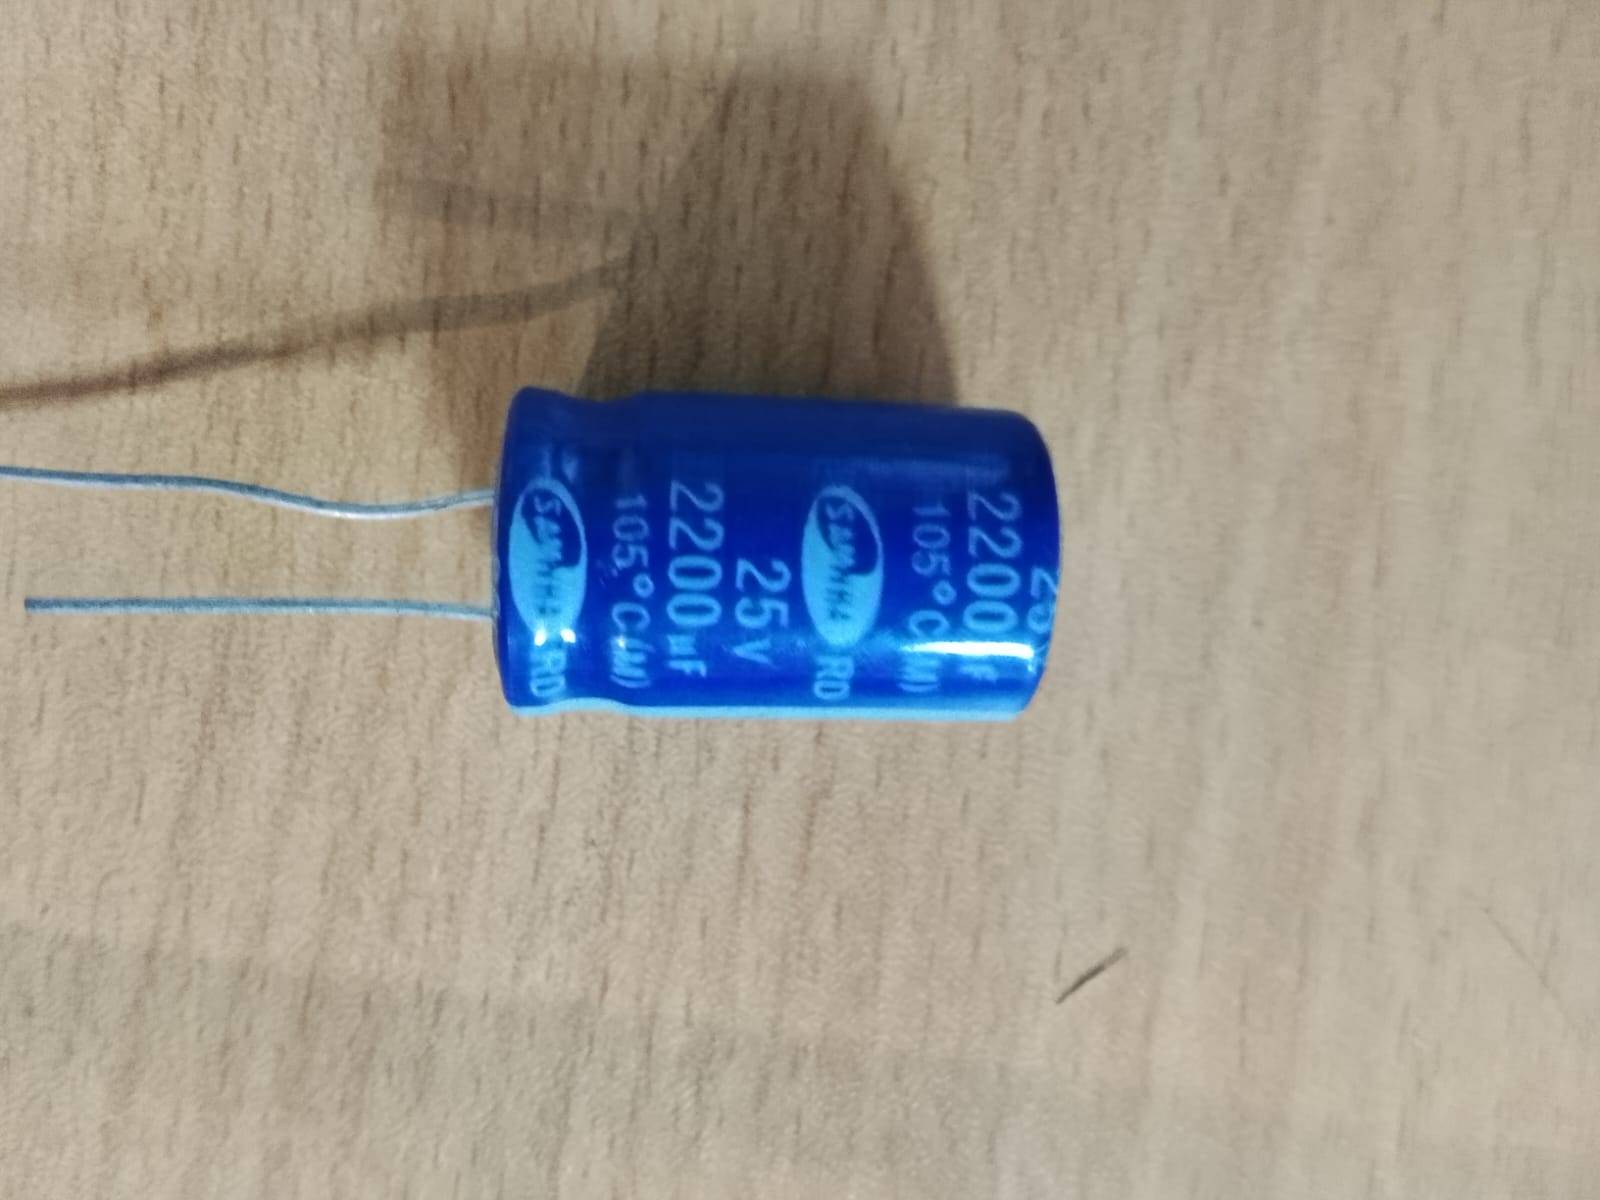
\includegraphics[width=\textwidth, height=5cm, keepaspectratio]{lab-01/assets/capacitor.jpeg}
    \caption{Electrolytic capacitors}
  \end{subfigure}
  \hfill
  \begin{subfigure}[b]{0.32\textwidth}
    \centering
    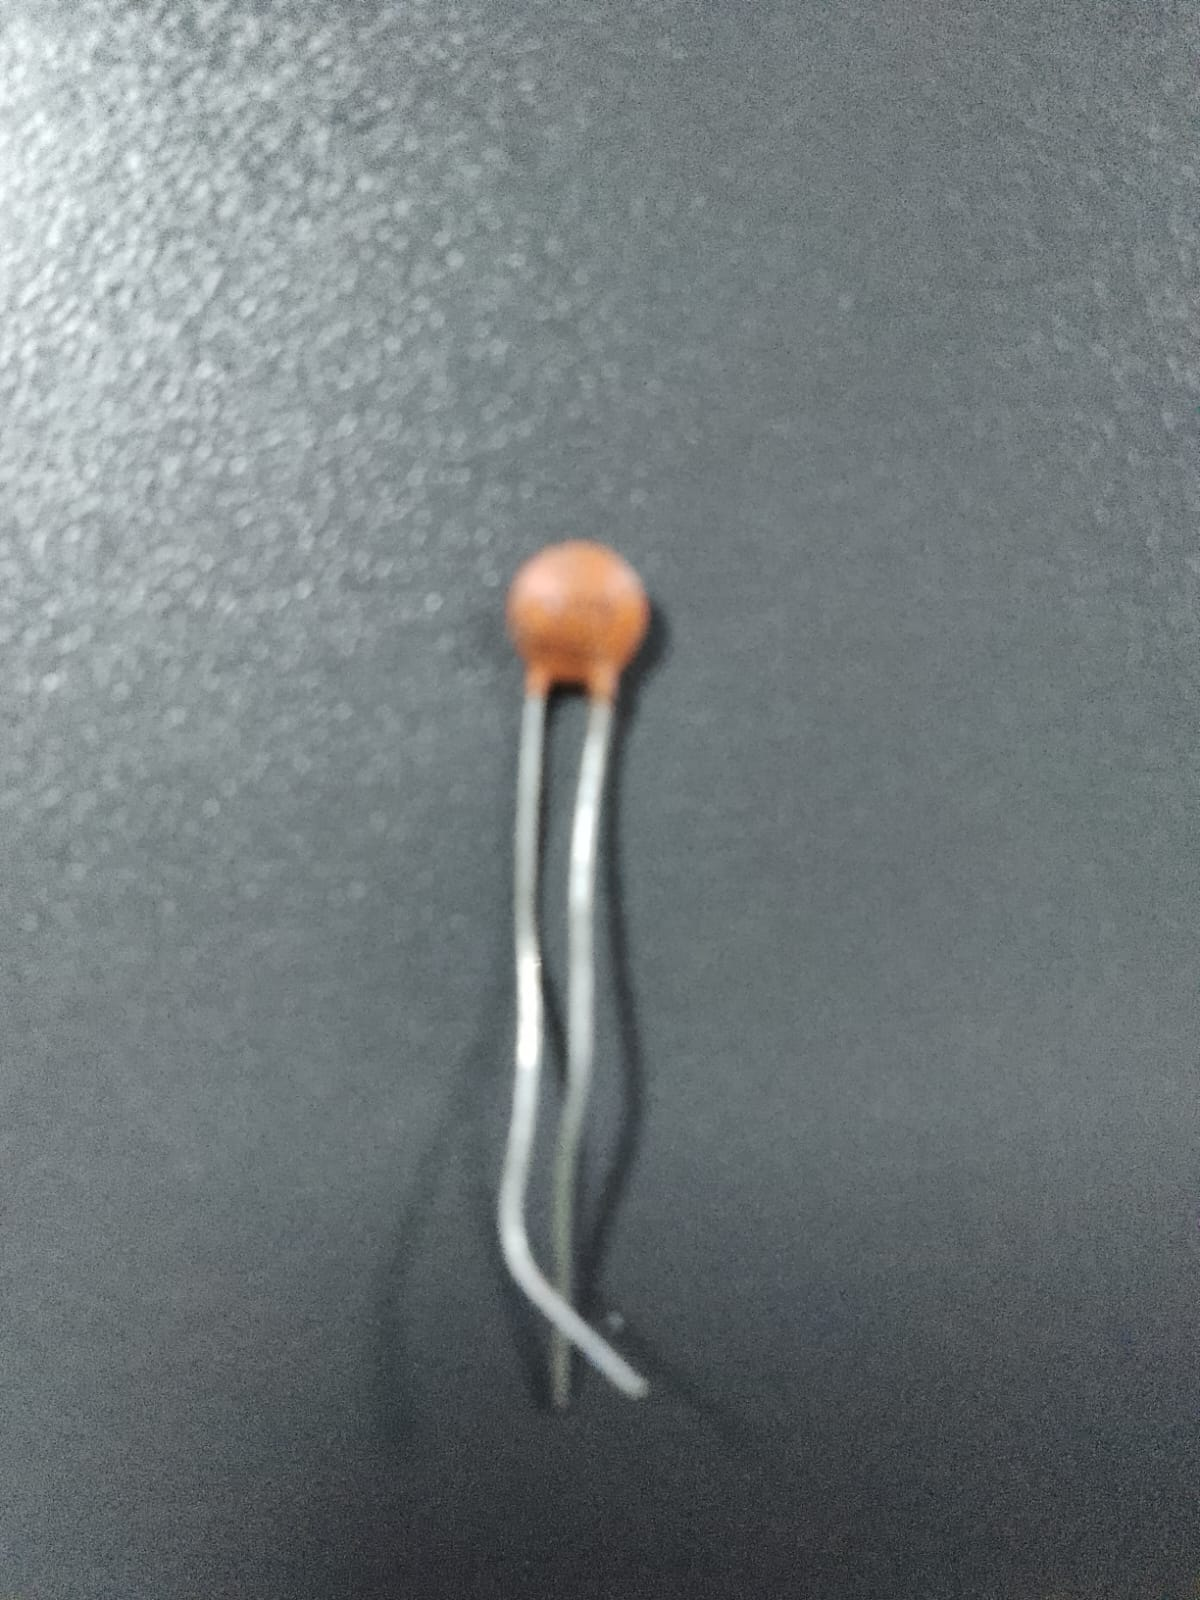
\includegraphics[width=\textwidth, height=5cm, keepaspectratio]{lab-01/assets/ceramic_capacitor.jpeg}
    \caption{Ceramic disc capacitor}
  \end{subfigure}
  \hfill
  \begin{subfigure}[b]{0.32\textwidth}
    \centering
    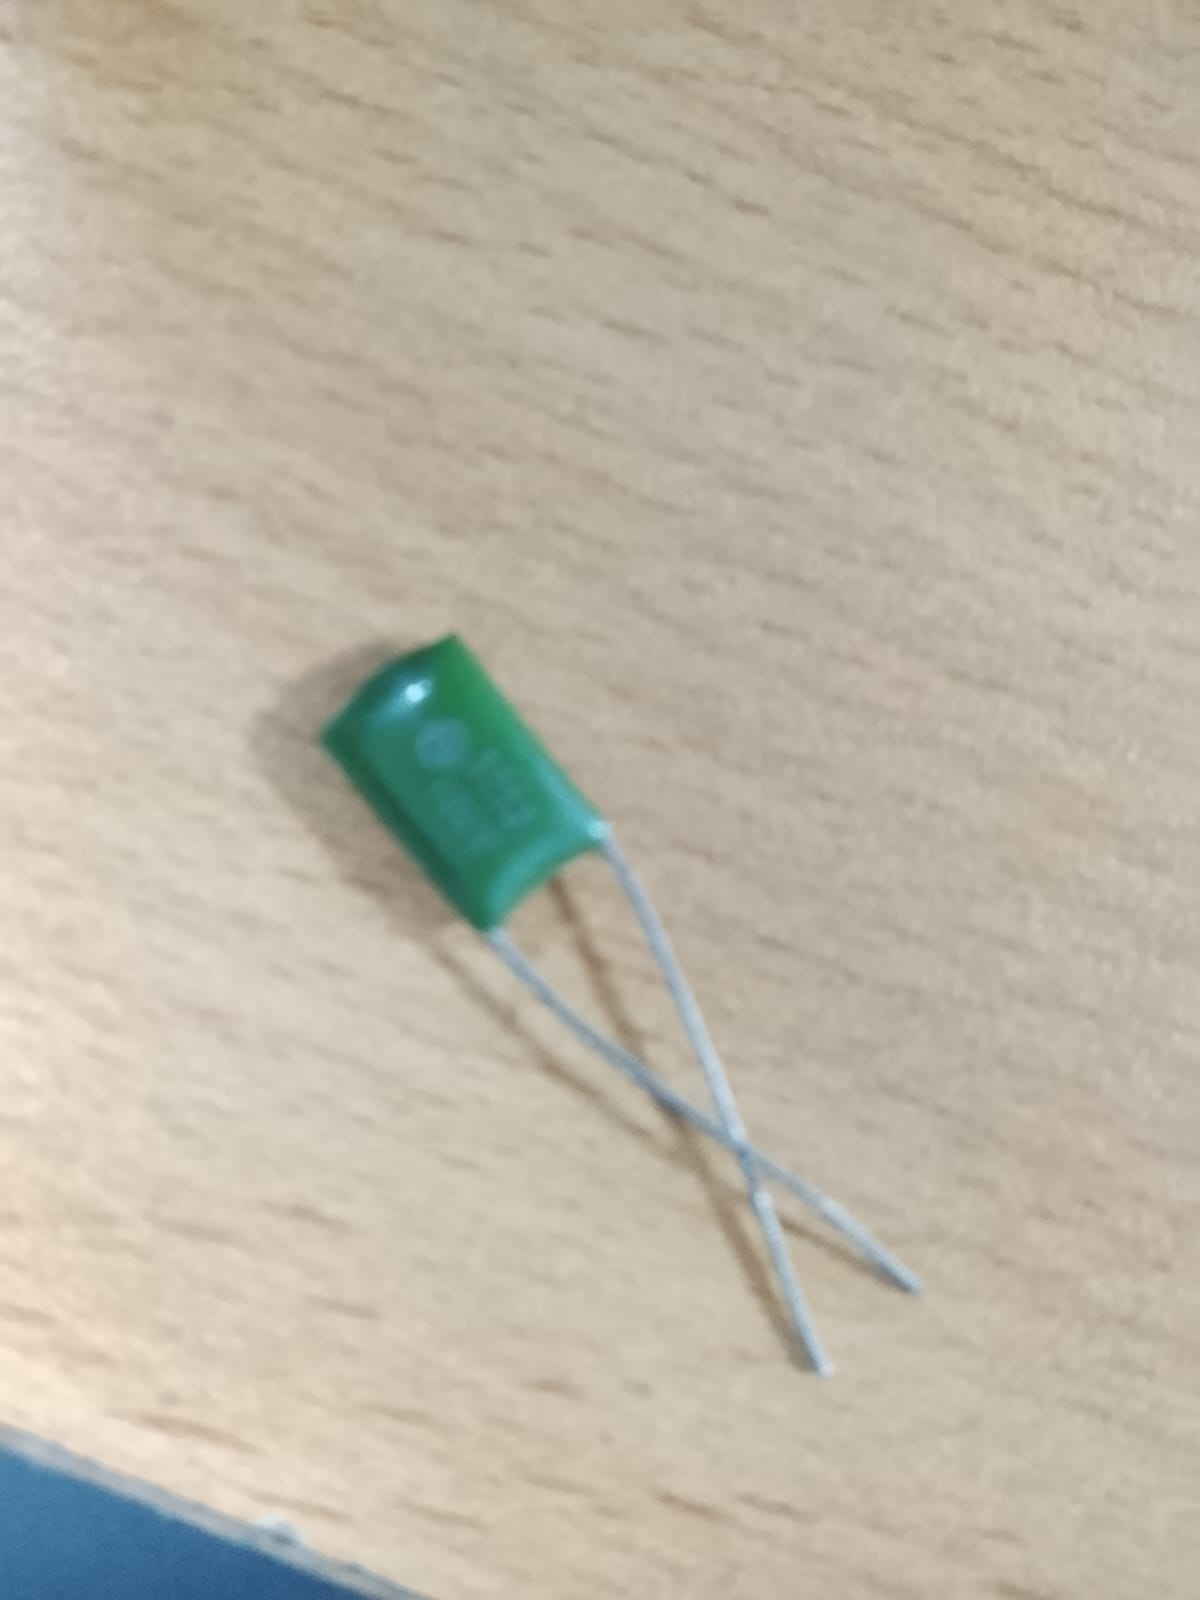
\includegraphics[width=\textwidth, height=5cm, keepaspectratio]{lab-01/assets/fim_capacitor.jpeg}
    \caption{Polyester film capacitor}
  \end{subfigure}
  \caption{Common capacitor types used in electronics laboratory work. The lab
           contains 2200\,$\mu$F/25\,V and 10\,$\mu$F/16\,V electrolytic units alongside
           ceramic disc and polyester film types.}
  \label{fig:capacitors_lab}
\end{figure}

\subsubsection*{Specifications}
Capacitance values span from femtofarads (ceramic chip, high-frequency bypass) to tens
of thousands of microfarads (aluminum electrolytic, power supply filtering). Critical
specifications include capacitance, voltage rating (maximum safe DC voltage), tolerance,
equivalent series resistance (ESR), leakage current, and temperature coefficient
\cite{boylestad2015}. Electrolytic types are polarized (must be connected with correct
polarity); ceramic, film, and tantalum types are available in non-polarized forms.

\subsubsection*{Purpose of Use}
Capacitors block DC while passing AC (coupling), smooth power supply ripple (filtering),
store charge for pulsed loads (energy storage), set oscillation frequencies in RC timing
circuits, and form resonant circuits with inductors for frequency selection.

\subsubsection*{Applications}
Capacitors are among the most commonly placed components in any circuit. Power supply
filter capacitors reduce ripple; decoupling capacitors suppress high-frequency noise on
IC power pins; coupling capacitors transfer audio or RF signals between stages; and
timing capacitors set delays and oscillation frequencies in astable circuits
\cite{horowitz2015}.

